

\section{Thiết kế phần cứng}

Hệ thống phần cứng được thiết kế hướng tới sự nhỏ gọn và tiết kiệm năng lượng, đồng thời cần đảm bảo năng lực tính toán đủ để thực thi song song các luồng xử lý tín hiệu và mạng nơ-ron.

\subsection{Nền tảng vi điều khiển lõi kép XIAO ESP32-S3}

Trung tâm điều khiển và xử lý suy luận của hệ thống là mô-đun Seeed Studio XIAO ESP32-S3. Việc lựa chọn nền tảng này thay vì các dòng vi điều khiển truyền thống được dựa trên ba yếu tố kỹ thuật chính:

\begin{itemize}
    \item Kiến trúc đa nhân và tập lệnh gia tốc Trí tuệ nhân tạo (AI): Chip được trang bị vi xử lý Xtensa® 32-bit LX7 lõi kép hoạt động ở xung nhịp 240 MHz. Dòng S3 có hỗ trợ các tập lệnh mở rộng vector, giúp thực thi các phép toán nhân-tích lũy (MAC) hiệu quả hơn, phù hợp cho việc gia tốc suy luận với mô hình TensorFlow Lite Micro \cite{ref_1_15}.
    \item Hệ thống bộ nhớ phân tầng: Hệ thống sử dụng phiên bản có tích hợp sẵn 8 MB PSRAM (Pseudo-Static RAM) và 8 MB bộ nhớ Flash bên cạnh 512 KB SRAM nội bộ \citeweb{ref_2_xiao}. Dung lượng PSRAM mở rộng đóng vai trò là vùng đệm cho phép hệ thống nạp cùng lúc ba mô hình mạng nơ-ron tự mã hóa (GENTLE, STRONG, SPIN), hỗ trợ thiết bị chuyển đổi mô hình linh hoạt mà không gây quá tải bộ nhớ.
    \item Kết nối Internet vạn vật (IoT): Tích hợp sẵn Wi-Fi 2.4 GHz, cung cấp băng thông đủ để triển khai các giao thức truyền tải mã hóa (WiFiClientSecure) kết nối với máy chủ đám mây.
\end{itemize}

\subsection{Tích hợp microphone kỹ thuật số INMP441 qua chuẩn giao tiếp I2S}

Để thu thập đặc trưng âm thanh, hệ thống sử dụng microphone kỹ thuật số đa hướng INMP441. Đây là cảm biến MEMS có các đặc điểm phù hợp với môi trường dễ nhiễu động như máy giặt:

\begin{itemize}
    \item Giao tiếp I2S (Inter-IC Sound): Tín hiệu âm thanh được số hóa trực tiếp tại cảm biến với độ phân giải 24-bit và truyền về vi điều khiển Seeed Studio XIAO ESP32-S3 qua bus I2S \cite{ref_2_inmp441}. Cách tiếp cận này giúp hạn chế nhiễu điện từ môi trường — một vấn đề thường gặp ở các microphone analog khi hoạt động gần động cơ công suất lớn.
    \item Cơ chế truy cập bộ nhớ trực tiếp (DMA): Luồng dữ liệu âm thanh lấy mẫu ở tần số 8 kHz được đẩy thẳng vào vùng nhớ SRAM thông qua bộ điều khiển DMA. Kỹ thuật này giúp hệ thống thu thập dữ liệu liên tục mà không làm tăng đáng kể tải xử lý của CPU, cho phép lõi số 0 tập trung tài nguyên vào khâu tính toán đặc trưng bộ lọc Mel.
\end{itemize}

\subsection{Tích hợp cảm biến gia tốc ADXL345 qua chuẩn giao tiếp I2C}

Sự rung động vật lý của lồng giặt là dữ liệu quan trọng để nhận diện các trạng thái bất thường cơ học. Cảm biến gia tốc ba trục ADXL345 được tích hợp với cấu hình như sau:

\begin{itemize}
    \item Độ phân giải và dải đo: Cảm biến được thiết lập ở dải đo $\pm$2g. Với độ phân giải 10-bit (tương đương mức độ nhạy 3,9 mg/LSB) \cite{ref_2_adxl345}, thiết bị có thể ghi nhận được các biến động nhỏ của lồng giặt, hỗ trợ thu thập dữ liệu đầu vào ổn định.
    \item Tốc độ lấy mẫu 1000 Hz: Cảm biến giao tiếp qua bus I2C và được gán mức ưu tiên cao nhất trong hệ điều hành FreeRTOS (mức ưu tiên 15). Việc duy trì chu kỳ lấy mẫu 1 ms/mẫu giúp hệ thống tính toán chính xác giá trị hiệu dụng và phương sai của trục Z, làm cơ sở dữ liệu cho thuật toán phân luồng trạng thái tự động.
\end{itemize}

\subsection{Sơ đồ kết nối và bố trí thiết bị trên đối tượng nghiên cứu}

Việc bố trí thiết bị giám sát được thiết kế dựa trên thực nghiệm, tuân thủ sơ đồ nối dây phần cứng chi tiết (Hình \ref{fig:hardware_wiring}).

\begin{figure}[H]
    \centering
    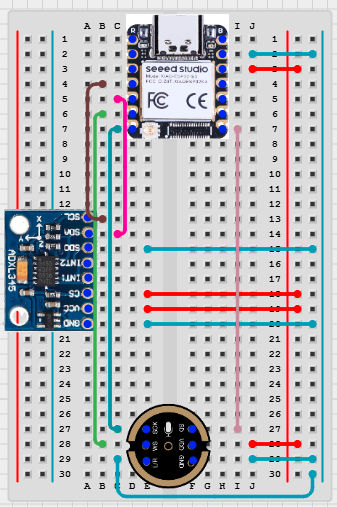
\includegraphics[width=0.3\linewidth]{chap2/image/SoDoNoiChan.png}
    \caption[Sơ đồ kết nối phần cứng]{Sơ đồ kết nối phần cứng và vị trí lắp đặt cụm cảm biến}
    \label{fig:hardware_wiring}
\end{figure}

Toàn bộ cụm mạch được đặt trong vỏ bảo vệ cách điện và gắn cố định tại mặt bên ngoài lồng giặt. Vị trí này được lựa chọn dựa trên hai yếu tố:
\begin{enumerate}
    \item Về mặt âm học: Hỗ trợ thu nhận tín hiệu âm thanh trực tiếp từ lồng máy, đồng thời giúp microphone giảm thiểu một phần các tạp âm nhiễu từ môi trường xung quanh.
    \item Về mặt cơ học: Các dao động do mất cân bằng tải hoặc lỗi trục sẽ được cảm biến gia tốc ghi nhận với biên độ rõ rệt nhất, qua đó cải thiện tỷ số tín hiệu trên nhiễu (SNR) của vector đặc trưng đầu vào.
\end{enumerate}

Với phần cứng và sơ đồ kết nối đã thiết lập, phần tiếp theo sẽ trình bày chi tiết về thiết kế phần mềm nhúng để điều phối các tác vụ và triển khai thuật toán Trí tuệ nhân tạo (AI) trên hệ thống.

% ==============================================================================
% DANH MỤC TÀI LIỆU THAM KHẢO TRÍCH DẪN (CHI TIẾT CHO MỤC 2.2)
% ==============================================================================
% \bibitem{ref_1_15} Espressif Systems, "ESP32-S3 Series Datasheet," Version 2.2, 2026.
% \bibitem{ref_2_xiao} Seeed Studio, "Getting Started with Seeed Studio XIAO ESP32S3 (Sense)," 2023. [Online]. Available: https://wiki.seeedstudio.com/xiao_esp32s3_getting_started/
% \bibitem{ref_2_inmp441} TDK InvenSense, "INMP441: Omnidirectional Microphone with Bottom Port and I2S Digital Output," Datasheet, 2014.
% \bibitem{ref_2_adxl345} Analog Devices, "3-Axis, ±2 g/±4 g/±8 g/±16 g Digital Accelerometer ADXL345," Datasheet, 2015.
